\subsection{Adding Functional Reactive Programming}
As shown in the first step, the need to handle $\Delta t$ explicitly can be quite messy, is inelegant and a potential source of errors, also the explicit handling of the state of an agent and its behavioural function is not very functional. We can solve both these weaknesses by switching to the functional reactive programming (FRP) paradigm, because it allows to express systems with discrete and continuous time-semantics. In this step we are focusing on arrowized FRP using the library Yampa. In it, time is handled implicit and cannot be messed with and the whole system is built on the concept of signal-functions (SF). A signal-function is basically a continuation which allows then to capture state using closures. Both these fundamental features allow us to tackle the weaknesses of our first step and push our approach further towards a truly functional approach.

We start by defining our agents now as a signal-function which receives the states of all agents as input and outputs the state of the agent:

\begin{minted}[fontsize=\footnotesize]{haskell}
type SIRAgent = SF [SIRState] SIRState 
\end{minted}

Now we can define the behaviour of an agent to be the following:

\begin{minted}[fontsize=\footnotesize]{haskell}
sirAgent :: RandomGen g => g -> SIRState -> SIRAgent
sirAgent g Susceptible = susceptibleAgent g
sirAgent g Infected    = infectedAgent g
sirAgent _ Recovered   = recoveredAgent
\end{minted}

Depending on the initial state we return one of three functions. Most notably is the difference that we are now passing a random-number generator instead of running in the Random Monad because signal-functions as implemented in Yampa are not capable of being monadic. We see that the recovered agent ignores the random-number generator which is in accordance with the implementation in the previous step where it acts as a sink which returns constantly the same state:

\begin{minted}[fontsize=\footnotesize]{haskell}
recoveredAgent :: SIRAgent
recoveredAgent = arr (const Recovered)
\end{minted}

The implementation of a susceptible agent in FRP is a bit more involved but much more expressive and elegant:

\begin{minted}[fontsize=\footnotesize]{haskell}
susceptibleAgent :: RandomGen g => g -> SIRAgent
susceptibleAgent g = 
    switch (susceptible g) (const (infectedAgent g))
  where
    susceptible :: RandomGen g => g -> SF [SIRState] (SIRState, Event ())
    susceptible g = proc as -> do
      makeContact <- occasionally g (1 / contactRate) () -< ()
      if isEvent makeContact
        then (do
          a <- drawRandomElemSF g -< as
          if (Infected == a)
            then (do
              i <- randomBoolSF g infectivity -< ()
              if i
                then returnA -< (Infected, Event ())
                else returnA -< (Susceptible, NoEvent))
            else returnA -< (Susceptible, NoEvent))
        else returnA -< (Susceptible, NoEvent)
\end{minted}

The implementation works as follows: the agent behaves as susceptible until it becomes infected, then it behaves as an infected agent by switching into the \textit{infectedAgent} SF.
Instead of randomly drawing the number of contacts to make we now follow a fundamentally different approach by using the \textit{occasionally} function. It generates on average an event after the given time, so in each time-step we generate either a single event or no event. This requires a fundamental different approach in selecting the right $\Delta t$ and sampling the system as will be shown in results. Note that we return an Event in case of an infection which indicates the switch into the new infected behaviour.

We deal with randomness different now and implement signal-functions built on the noiseR function provided by Yampa. This function takes a range of values and the random-number generator as input and returns the \textit{next} value in the range. This is another example of the statefulness of a signal-function as it needs to keep track of the changed random-number generator internally through the use of continuations and closures. Here we provide the implementation of \textit{randomBoolSF}, drawRandomElemSF works similar but takes a list as input:

\begin{minted}[fontsize=\footnotesize]{haskell}
randomBoolSF :: RandomGen g => g -> Double -> SF () Bool
randomBoolSF g p = proc _ -> do
  r <- noiseR ((0, 1) :: (Double, Double)) g -< ()
  returnA -< (r <= p)
\end{minted}

Implementing the infected agent in FRP is also a bit more involved but much more expressive too:

\begin{minted}[fontsize=\footnotesize]{haskell}
infectedAgent :: RandomGen g => g -> SIRAgent
infectedAgent g = 
    switch infected (const recoveredAgent)
  where
    infected :: SF [SIRState] (SIRState, Event ())
    infected = proc _ -> do
      recEvt <- occasionally g illnessDuration () -< ()
      let a = event Infected (const Recovered) recEvt
      returnA -< (a, recEvt)
\end{minted}

The infected agent behaves as infected until it recovers on average after the illness duration after which it behaves then as a recovered agent by switching into \textit{recoveredAgent}. As in the susceptible agent we use the occasionally function to generate the event when the agent recovers. Note that the infected agent ignores the states of the other agents as its behaviour is completely independent of them.

Running and stepping the simulation works now a bit different:

\begin{minted}[fontsize=\footnotesize]{haskell}
runSimulation :: RandomGen g => g -> Time -> DTime -> [SIRState] -> [[SIRState]]
runSimulation g t dt as = embed (stepSimulation sfs as) ((), dts)
  where
    steps = floor (t / dt)
    dts = replicate steps (dt, Nothing)
    n = length as
    (rngs, _) = rngSplits g n [] -- creates unique RandomGens for each agent
    sfs = map (\ (g', a) -> sirAgent g' a) (zip rngs as)
\end{minted}

Yampa provides the function \textit{embed} which allows to run a signal-function for a given number of steps where in each step one provides the $\Delta t$ and an optional input. What we now need to implement is a closed feedback-loop. Fortunately there exists research \cite{nilsson_functional_2002}, \cite{courtney_yampa_2003} which discusses implementing this in Yampa. The function \textit{stepSimulation} is an implementation of such a closed feedback-loop:

\begin{minted}[fontsize=\footnotesize]{haskell}
stepSimulation :: [SIRAgent] -> [SIRState] -> SF () [SIRState]
stepSimulation sfs as =
    dpSwitch
      (\_ sfs' -> (map (\sf -> (as, sf)) sfs'))
      sfs
      (switchingEvt >>> notYet) 
      stepSimulation
  where
    switchingEvt :: SF ((), [SIRState]) (Event [SIRState])
    switchingEvt = arr (\ (_, newAs) -> Event newAs)
\end{minted}

This function takes all the signal-functions and current states of all agents and returns a signal-function which has the unit-type as input and returns a list of agent-states. What we need to do is to run all agents signal-functions in parallel where all the agent-states are passed as inputs and collect the output of all signal-functions into a list. Fortunately Yampa provides the function \textit{dpSwitch} for this task. (TODO: explain the d in p, and why we use it: delay guarantees that we delay the switching until the next time e.g. the function into which we switch is only applied in the next step). Its first argument is the pairing-function which pairs up the input to the signal-functions, the second argument is the collection of signal-functions, the third argument is a signal-function generating the switching event and the last argument is a function which generates the continuation after the switching event has occurred.
dpSwitch then returns a new signal-function which runs all the signal-functions in parallel (thus the p) and switching into the continuation when the switching event occurs. The continuation-generation function gets passed the signal-functions after they were run in parallel and the data of the switching event which in combination allows us to recursively switch back into the stepSimulation function. In every step we generate a switching event which passes the final agent-states to the continuation-generation which in turn simply returns stepSimulation recursively but now with the new signal-functions and the new agent-states. Note the need for \textit{notYet} which is required because at $t = 0$ switching occurs immediately. If we would omit this we would enter an infinite recursion at $t = 0$ which can be broken by the use of notYet. 

\subsubsection{Results}
As already mentioned, because we are now using the occasionally function we need a different approach of sampling the system. In the infected agent occasionally determines the time when an agent recovers so its a discrete transition but in a susceptible agent it determines the average number of contacts per time unit: it is a rate with an exponential distribution. This requires us to sample the system with small enough $\Delta t$ to arrive at the correct solution - if we choose a too large $\Delta t$, we loose events which will result in dynamics which do not approach the SD dynamics.
We investigated the behaviour of occasionally under varying $\Delta t$, which we added as Appendix TODO add appendix. From this it becomes apparent that we need to step our simulation with a $\Delta t <= 0.1$ to arrive at a sufficiently close approximation of the SD dynamics.

TODO: show results
\begin{figure}
	\centering
	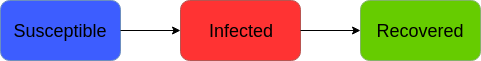
\includegraphics[width=.4\textwidth, angle=0]{./fig/step2_yampa/SIR_transitions.png}
	\caption{Transitions in the SIR compartment model.}
	\label{fig:sir_transitions}
\end{figure}

TODO: ALARM ALARM !!!! our dynamics do not approach the ones of SD yet, Step 1 solution is much better, probably because we need supersampling! when reducing time-deltas to 0.001 we arrive at good solutions.
TODO: compare the results to random-monad solution 100 agents. with smaller and smaller time-delta we need only 1 infected agent and arrive already at a good approximation. this is not the case in random-monad where because of 1.0 time-delta it results in too non fine-grained resolution

By moving on to FRP using Yampa we made a huge improvement in clarity, expressivity and robustness of our implementation. Also by using explicit time-semantics with \textit{occasionally} we can achieve extremely fine grained stochastics: as opposed to draw random number of events we create only a single event or not. This requires then to sample the system with a much smaller $\Delta t$: we are treating it as a truly continuous system. Still we are not too happy about our approach as we feed back all agents states into every agent, something we want to omit in an agent-based simulation. We now move on to step 3 in which we introduce a more general and much more controlled mechanism for feeding back agent-states. State is now implicit!